\documentclass[11pt,]{article}
\usepackage{lmodern}
\usepackage{amssymb,amsmath}
\usepackage{ifxetex,ifluatex}
\usepackage{fixltx2e} % provides \textsubscript
\ifnum 0\ifxetex 1\fi\ifluatex 1\fi=0 % if pdftex
  \usepackage[T1]{fontenc}
  \usepackage[utf8]{inputenc}
\else % if luatex or xelatex
  \ifxetex
    \usepackage{mathspec}
  \else
    \usepackage{fontspec}
  \fi
  \defaultfontfeatures{Ligatures=TeX,Scale=MatchLowercase}
\fi
% use upquote if available, for straight quotes in verbatim environments
\IfFileExists{upquote.sty}{\usepackage{upquote}}{}
% use microtype if available
\IfFileExists{microtype.sty}{%
\usepackage{microtype}
\UseMicrotypeSet[protrusion]{basicmath} % disable protrusion for tt fonts
}{}
\usepackage[margin=1in]{geometry}
\usepackage{hyperref}
\hypersetup{unicode=true,
            pdftitle={raptr: Representative and Adequate Prioritization Toolkit in R},
            pdfborder={0 0 0},
            breaklinks=true}
\urlstyle{same}  % don't use monospace font for urls
\usepackage{graphicx,grffile}
\makeatletter
\def\maxwidth{\ifdim\Gin@nat@width>\linewidth\linewidth\else\Gin@nat@width\fi}
\def\maxheight{\ifdim\Gin@nat@height>\textheight\textheight\else\Gin@nat@height\fi}
\makeatother
% Scale images if necessary, so that they will not overflow the page
% margins by default, and it is still possible to overwrite the defaults
% using explicit options in \includegraphics[width, height, ...]{}
\setkeys{Gin}{width=\maxwidth,height=\maxheight,keepaspectratio}
\IfFileExists{parskip.sty}{%
\usepackage{parskip}
}{% else
\setlength{\parindent}{0pt}
\setlength{\parskip}{6pt plus 2pt minus 1pt}
}
\setlength{\emergencystretch}{3em}  % prevent overfull lines
\providecommand{\tightlist}{%
  \setlength{\itemsep}{0pt}\setlength{\parskip}{0pt}}
\setcounter{secnumdepth}{0}

%%% Use protect on footnotes to avoid problems with footnotes in titles
\let\rmarkdownfootnote\footnote%
\def\footnote{\protect\rmarkdownfootnote}

%%% Change title format to be more compact
\usepackage{titling}

% Create subtitle command for use in maketitle
\newcommand{\subtitle}[1]{
  \posttitle{
    \begin{center}\large#1\end{center}
    }
}

\setlength{\droptitle}{-2em}
  \title{raptr: Representative and Adequate Prioritization Toolkit in R}
  \pretitle{\vspace{\droptitle}\centering\huge}
  \posttitle{\par}
  \author{Jeffrey O. Hanson\(^1\), Jonathan R. Rhodes\(^2\), Hugh P.
Possingham\(^{1,3}\), Richard A. Fuller\(^1\)\\
\(^1\)School of Biological Sciences, The University of Queensland,
Brisbane, QLD, Australia\\
\(^2\)School of Earth and Environmental Sciences, The University of
Queensland, Brisbane, QLD, Australia\\
\(^3\)The Nature Conservancy, South Brisbane, QLD, Australia\\
Correspondence should be addressed to
\href{mailto:jeffrey.hanson@uqconnect.edu.au}{\nolinkurl{jeffrey.hanson@uqconnect.edu.au}}}
  \preauthor{\centering\large\emph}
  \postauthor{\par}
  \predate{\centering\large\emph}
  \postdate{\par}
  \date{06 April 2017}

% load packages
\usepackage{amsmath,amsfonts,float,makecell,titletoc,titlesec,tocloft,lineno,booktabs,subfiles}
\usepackage[T1]{fontenc}
\usepackage{lmodern}
\usepackage[utf8]{inputenc}
\usepackage[doublespacing]{setspace}

% format captions
\usepackage[labelfont={small,bf}, labelsep=space, font={small}]{caption}

% line numbers
\linenumbers

% allow breaks in equations
\allowdisplaybreaks

% format abstract
\renewcommand{\abstractname}{Summary}
\renewenvironment{abstract}
 {\small
  \begin{center}
  \bfseries \abstractname\vspace{-.5em}\vspace{0pt}
  \end{center}
  \list{} {%
   \setlength{\leftmargin}{2mm}
   \setlength{\rightmargin}{\leftmargin}%
  }%
  \item\relax}
{\endlist}

% format section headers
\titleformat*{\section}{\Large\bfseries}
\titleformat{\subsection}[display]
	{\large\sffamily\lsstyle}
	{\subsectiontitlename\ \thesubsection}
	{0.5em}{}
\titleformat*{\subsubsection}{\large\itshape}

% make figures static
\let\origfigure\figure
\let\endorigfigure\endfigure
\renewenvironment{figure}[1][2] {
	\expandafter\origfigure\expandafter[H]
} {
	\endorigfigure
}

% define struts for tables
\newcommand\T{\rule{0pt}{2.6ex}} % top strut
\newcommand\B{\rule[-1.2ex]{0pt}{0pt}} % bottom strut

% define command to put new lines in table cells
%\newcommand{\specialcell}[2][c]{%
%  \begin{tabular}[#1]{@{}c@{}}#2\end{tabular}}

\begin{document}
\maketitle

Abstract word count: 347 / 350\\
Total word count: XXXX / 7000\\
Number of references: 42\\
Number of figures: 8\\
Number of tables: 0\\
Number of textboxes: 0\\
Number of equations: 4\\
Short running title: Short abstract: Prioritize biodiversity processes
and patterns using raptr \url{https://github.com/jeffreyhanson/raptr}\\
Keywords: conservation, biodiversity, mixed integer linear programming,
optimization, protected areas

\clearpage

\section{Summary}\label{summary}

\begin{enumerate}
\def\labelenumi{\arabic{enumi}.}
\item
  An underlying aim in conservation planning is to maximize the
  long-term persistence of biodiversity. To fulfill this aim, the
  ecological and evolutionary processes that sustain biodiversity must
  be preserved. One way to conserve such processes at the feature level
  (eg. species, ecosystem) is to preserve a sample of the feature (eg.
  individuals, areas) that is representative in terms of the intrinsic
  or extrinsic physical attributes that underpin the process of
  interest. For example, by conserving a sample of populations with
  local adaptations that is representative in terms of the full
  variation found in the species--physical attributes associated with
  adaptation--protected areas can foster adaptive processes by ensuring
  these adaptations are not lost. Despite this, current reserve
  selection methods overwhelmingly focus on securing an adequate amount
  of area or habitat for each feature. Little attention has been
  directed towards capturing a representative sample of each feature.
\item
  To address this issue, we developed the \texttt{raptr R} package to
  help guide reserve selection. Users set ``amount targets''--similar to
  conventional methods--to ensure that solutions secure a sufficient
  proportion of area or habitat for each feature. Additionally, users
  set ``space targets'' to secure a representative sample of variation
  in ecologically or evolutionary relevant attributes (eg. environmental
  or genetic variation). We demonstrate the functionality of this
  package using simulations and two case studies. In these studies, we
  generated solutions using amount targets--representing conventional
  methods--and compared them with solutions generated using amount and
  space targets.
\item
  Our results demonstrate that different solutions emerge when targeting
  a representative sample of each feature. We show that using these
  targets is important for features that have multimodal distributions
  in the process-related attributes (eg. species with multimodal
  niches). We also found that solutions could conserve a far more
  representative sample with only a slight increase in reserve size.
\item
  The \texttt{raptr R} package provides a toolkit for making
  prioritizations that secure an adequate and representative sample of
  each feature. By using solutions that secure a representative sample
  of each feature, prioritizations may have a greater chance of
  achieving long-term biodiversity persistence.
\end{enumerate}

\clearpage
\section{Introduction}\label{introduction}

Perhaps the most fundamental aim of conservation is to maximize the
long-term persistence of biodiversity (McNeely 1994; Margules \& Pressey
2000). To achieve this, conservation actions must preserve biodiversity
patterns (eg. populations, species, ecosystems), but also crucially the
processes that sustain them. One of the major tangible achievements of
modern conservation has been the act of setting aside areas for
preservation (Watson \emph{et al.} 2014; Sanderson \emph{et al.} 2015).
Reserve networks buffer species from gross threatening processes and set
the stage for enhanced management interventions (Gaston \emph{et al.}
2008). Since the resources available for conservation action are
limited, protected area networks must be sited in places that satisfy
conservation objectives for minimal cost (Margules \& Pressey 2000).

Today, the most widely used conservation planning tools focus on
biodiversity patterns (\texttt{Zonation} and \texttt{Marxan}; Moilanen
2007; Ball \emph{et al.} 2009). Decision makers can use these tools to
obtain solutions that secure a proportion of the geographic range of
each biological feature (populations, species, or ecosystems) of
interest by setting targets. One method to incorporate data on the
ecological and evolutionary processes that sustain biological features
is to conserve a representative sample of the physical attributes that
underpin these processes. To achieve this, current methods typically
involve partitioning each feature into sub-groups based on an attribute
variable that relates to a biodiversity process of interest (Cowling \&
Pressey 2001; Pyke \& Fischer 2005; Klein \emph{et al.} 2009). For
instance, by dividing species distributions into sub-groups according to
habitat discontinuities, and ensuring that each sub-group is represented
in the solution, conservation planners can obtain prioritizations that
promote adaptive processes (Carvalho \emph{et al.} 2011). However, using
this method is challenging because biodiversity often cannot be divided
into operational groups for conservation planning without loss of
information (Orians 1993; Pressey \& Logan 1994; Faith \& Walker 1996).
This limitation has been known of quite some time, and dates back to
some of the earliest reserve selection methods (Orians 1993).

To overcome this limitation, Faith and Walker (1993) developed a
decision support tool (\texttt{DIVERSITY}) to identify prioritizations
that secure a representative sample of the environmental variation found
across a study area. Although this method was originally pitched as an
alternative to species-based conservation planning (Faith 1994, 2003;
Faith \& Walker 1996), it can also identify solutions that conserve a
representative sample of variation across a single species' range.
Recent work has built on this reserve selection method by solving
problems with more advanced optimization algorithms (Engelbrecht
\emph{et al.} 2016). However, existing \texttt{DIVERSITY}-based methods
have limited utility for species-based conservation planning, in part,
because they cannot accommodate multiple biological features and do not
provide options to specify specific targets pertaining to the amount of
habitat required to conserve species (unlike \texttt{Marxan} and
\texttt{Zonation}). As a consequence, such methods are not useful for
most conservation planning exercises (Margules \& Pressey 2000).

Conservation planners lack a decision support tool that lets them set
explicit targets to obtain solutions that (1) secure an adequate amount
of habitat for each feature and (2) a representative sample of the
variation in each feature. To begin to fill this gap, here we unite the
ideas underpinning \texttt{DIVERSITY} and \texttt{Marxan} into new
formulations of the reserve selection problem, and implement them in the
\texttt{raptr R} package. This \texttt{R} package provides decision
makers with the tools to generate prioritizations based on data that
relate to biodiversity patterns and processes. Here, we aim to the
provide an in-depth understanding of this \texttt{R} package and explore
its functionality.

\section{Methods}\label{methods}

\subsection{PROBLEM FORMULATION}\label{problem-formulation}

Biodiversity features are defined as the entities that the
prioritization is required to preserve (eg. species, ecosystems). Here,
attributes are defined as the variation across the features' ranges that
the prioritization is required to sample. These attributes can be
intrinsic (eg. genetic or phenotypic) or extrinsic (eg. environmental
conditions) to the feature. There should, however, be a reasonable
underlying hypothesis that relates the attribute to the biodiversity
processes that needs to be conserved.

A set of attributes is conceptualized as a space (termed an ``attribute
space''). For example, a decision maker may require a prioritization
that represents populations along climatic gradients. To achieve this,
the decision maker might use a ``climatic'' attribute space with
dimensions relating to mean annual temperature (\(^{\circ}\)C) and
precipitation (mm). Any given combination of temperature and
precipitation may be conceived as a point in this climatic space.
Although they exist as polygons, for simplicity, each planning unit may
be thought to exist as a single point inside a given attribute space. By
associating the planning units with climatic data, and calculating a
descriptive statistic for each planning unit (eg. mean), they can be
mapped from geographic space to this climatic attribute space. In
addition to points representing planning units, attribute spaces also
contain demand points.

Demand points (Faith \& Walker 1993, 1996; Faith 2003) are designated by
the decision maker to indicate regions of the attribute space that they
wish to represent in the prioritization (see below for discussion on
generating demand points for real-world data sets). For instance, by
siting demand points throughout an attribute space, planners can obtain
solutions that conserve a representative sample of an attribute space.
Alternatively, by siting demand points in specific regions of an
attribute space, planners can obtain solutions that target specific
samples of an attribute space. For a given set of demand points, the
shorter the distances between the demand points and the planning units
selected for prioritization; the better a solution is at securing the
desired variation in the attribute space. In any attribute space there
may exist points that are impossible (eg. mean annual rainfall -5 mm),
or do not occur in the study area (eg. mean annual temperature
30\(^{\circ}\)C in Antarctica). Additionally, there may be some regions
that are desirable for some features and undesirable for others (eg.
conditions known to be outside the physiological tolerance of certain
species). Thus a different set of demand points may be appropriate for
different attribute spaces and features.

To illustrate these concepts, consider the following example: we wish to
develop a prioritization for a single species that has four populations.
Since we can only afford to preserve three of the four populations, our
objective is to conserve the most representative sample possible. To
achieve this goal, we obtained annual rainfall (mm) and temperature
(\(^{\circ}\)C) data at the location of each population. We used this
data to construct a two-dimensional climatic attribute space. Next, we
generated demand points as equi-distant points inside this space. By
comparing the distribution of the demand points to the distribution of
the populations in the attribute space, we can identify the optimal
solution (Fig. 1). We can see that a solution that prioritizes both
populations \emph{A} and \emph{B}, effectively ``doubles-up'' on the
same climatic characteristics and constitutes considerable redundancy if
both selected. Instead, a more representative sample of the
intra-specific variation could be captured by securing populations
\emph{A} (or \emph{B}), \emph{C}, and \emph{D}. However, if the goal of
the prioritization was to preserve populations living in warmer
temperatures, then instead of siting demand points across the full range
of conditions, we could site demand points in environmental conditions
with temperatures over 30 \(^{\circ}\)C (ie. the top two rows of demand
points in Fig. 1). Given this new set of demand points, populations
\emph{A}, \emph{B}, and \emph{C} would be prioritized. Since demand
points can be sited and weighted in any configuration, they provide a
flexible means to guide the reserve selection process.

The \texttt{raptr R} package utilizes two novel formulations of reserve
selection problem to generate prioritizations. These formulations are
based on elements of the \texttt{Marxan}, \texttt{DIVERSITY}, and
uncapacitated facility location problems (Cornuéjols \emph{et al.}
1990). Since they are based on the unreliable and reliable facility
location problems (Cui \emph{et al.} 2010), the formulations are
hereafter referred to as the ``unreliable'' and ``reliable''
formulations. The difference between the two formulations is that the
reliable formulation explicitly considers the probability that planning
units are occupied by features when calculating how well a given
solution samples a feature's attribute space. On the other hand, the
unreliable formulation assumes that features occupy all of the planning
units within which they are found with 100 \% certainty when performing
these calculations. For brevity, we will define the simpler
formulation--the unreliable formulation--below and define the more
complex version--the reliable formulation--in Appendix S1. All
mathematical terms defined hereafter are described in Table S1. For
convenience, the cardinality of sets will be denoted using the same
symbol used to denote the set.

Define \(F\) to be the set of features one wishes to conserve (indexed
by \(f\)). Let \(J\) be a set of planning units (indexed by \(j\)).
Also, let \(A_j\) denote the area, and \(C_j\) denote the cost of
preserving planning unit \(j \in J\). To assess the extent to which each
feature is secured in a given prioritization, let \(q_{fj}\) denote the
probability of feature \(f\) occupying planning unit \(j\). The level of
fragmentation associated with a prioritization is parameterized as the
total exposed boundary length (as in \texttt{Marxan}). Let the shared
edges between each planning unit \(j \in J\) and \(k \in J\) be
\(e_{jk}\).

Let \(S\) denote a set of attribute spaces (indexed by \(s\)). Each
\(j \in J\) is associated with spatially explicit data that represent
coordinates for each attribute space \(s \in S\). Let \(I_{fsi}\) denote
a set of demand points (indexed by \(i\)) for each feature \(f \in F\)
and each attribute space \(s \in S\). Let \(\lambda_{fsi}\) denote the
weighting for each demand point \(i \in I\), \(f \in F\) and
\(s \in S\). Let \(d_{fsij}\) denote the distance between each demand
point \(i \in I\) and each planning unit \(j \in J\) for each feature
\(f \in F\) and attribute space \(s \in S\). To describe the inherent
variation in the distribution of demand points for feature \(f\) and
space \(s\), let \(\delta_{fsi}\) denote the distance between each
demand point \(i \in I\) and the centroid of the demand points. Demand
points with greater weight \(\lambda_{fsi}\) are more important, and the
solutions that select planning units close to highly weighted demand
points will be more favorable. As a consequence, the decision maker will
need to choose an appropriate weighting for each demand point.

Targets are used to ensure that prioritizations sufficiently conserve
each feature. Amount-based targets specify the minimum amount of habitat
required for each feature to be adequately conserved (similar to those
used in \texttt{Marxan}). Let \(T_f\) denote the amount of area or
habitat that needs to be preserved for each feature \(f \in F\).
Space-based targets specify the minimum proportion of variation in the
demand points that needs to be secured for each feature to be
sufficiently conserved. Space-based targets are expressed as
proportions--instead of a sum of weighted distances--by scaling the sum
of weighted distances between the demand points and the selected
planning units in a solution relative to the distances between demand
points and the demand points' centroid. This scaling is conceptually
similar to that used in calculating the R\(^2\) statistic for
\emph{K}-means clustering analyses from the within sums of squares and
total sums of squares {[}Greenacre \& Primicerio (2014); page 106{]}.
Let \(\tau_{fs}\) denote the space-based targets for feature \(f \in F\)
and attribute space \(s \in S\). The control variables for the
unreliable formulation are the \(B\), \(T_{s}\), and \(\tau_{fs}\)
variables.

\begin{align*}
T_s &= \text{amount target for feature $f$} \tag*{eqn 1a}\\
%
\tau_{fs} &= \parbox{25em}{space target for feature $f$ in attribute space $s$} \tag*{eqn 1b}\\
%
B &= \text{boundary length modifier (BLM) to penalize fragmented solutions} \tag*{eqn 1c}\\
\end{align*}

The decision variables are the \(X_j\) and \(Y_{fsij}\) variables.

\begin{align*}
X_j
  &= \begin{cases}
    1, & \parbox{25em}{if planning unit $j$ is selected for conservation action} \tag*{eqn 2a} \\
    0, & \parbox{25em}{otherwise} \\
  \end{cases} \\
%
Y_{fsij} &= \begin{cases}
    1, & \parbox{25em}{if demand point $i$ is used to represent planning unit $j$ for feature $f$ in space $s$. } \tag*{eqn 2b} \\
    0, & \parbox{25em}{otherwise} \\
  \end{cases} \\
\end{align*}

Each demand point \(i \in I\) for feature \(f \in F\) and space
\(s \in S\) is represented by a single selected planning unit (ie. a
\(j \in J\) where \(X_j = 1\)). The degree to which a demand point \(i\)
is represented by a planning unit \(j\) is determined by the distance
between them (\(d_{fsij}\)). Generally--unless near zero space targets
are used so that the problem is effectively unconstrained by the
target--demand points are represented by their closest selected planning
units. In poorer quality solutions, demand points will be represented by
planning units that have larger distances between them. As a
consequence, the sum of the weighted distances between all of the demand
demand points and the planning units used to represent them will be
larger, and so, the solution will capture less of the variation
described by the demand points.

The unreliable formulation (URAP) is a defined as a multi-objective
optimization problem.

\begin{align*}
& \text{(URAP)} & \text{Min } & \sum_{j=0}^{J-1} \left( X_j C_j \right) + \sum_{j=0}^{J-1} \sum_{k=j}^{J-1} X_j \left( 1-X_k \right) \left( B e_{jk} \right) + & & \tag*{eqn 3a} \\
%
& & \text{s.t. } & \sum_{j=0}^{J-1} A_j q_{fj} \geq T_{f} & \forall & 0 \leq f \leq F-1 \tag*{eqn 3b}\\
%
& & & 1 - \frac{\sum_{i=0}^{I-1} \sum_{j=0}^{J-1} \lambda_{fsi} {d_{fsij}}^{2} Y_{fsij}}{\sum_{i=0}^{I-1} \lambda_{fsi} {\delta_{fsi}}^{2}} \geq \tau_{fs} & \forall & 0 \leq f \leq F-1, \tag*{eqn 3c}\\
& & & & & 0 \leq s \leq S-1\\
%
& & & \sum_{j=0}^{J-1} Y_{fsij} = 1 & \forall & 0 \leq f \leq F-1, \tag*{eqn 3d}\\
& & & & & 0 \leq s \leq S-1, \\
& & & & & 0 \leq i \leq I-1\\
%
& & & Y_{fsij} \leq X_j & \forall & 0 \leq f \leq F-1, \tag*{eqn 3e}\\
& & & & & 0 \leq s \leq S-1, \\
& & & & & 0 \leq i \leq I-1,\\
& & & & & 0 \leq j \leq J-1\\
%
& & & X_j, Y_{fsij} \in {0,1} & \forall & 0 \leq f \leq F-1, \tag*{eqn 3f}\\
& & & & & 0 \leq s \leq S-1,\\
& & & & & 0 \leq i \leq I-1\\
%
\end{align*}

The objective function (eqn 3a) determines the utility of a given
prioritization: a combination of the total cost of a prioritization and
how fragmented it is. Constraints (eqn 3b) ensure that all the
amount-based targets are met. Constraints (eqn 3c) ensure that all the
space-based targets are met for each feature and each attribute space.
For each feature and attribute space, the total weighted distance
between the demand points and their closest selected planning units is
calculated
(\(\sum_{i=0}^{I-1} \sum_{j=0}^{J-1} \lambda_{fsi} {d_{fsij}}^{2} Y_{fsij}\)).
This total weighted distance is then scaled by the inherent variation in
the demand points
(\(\sum_{i=0}^{I-1} \lambda_{fsi} {\delta_{fsi}}^{2}\)). As previously
mentioned, the resulting fraction is used to calculate a proportion
conceptually similar to the \(R^2\) statistic used in \(k\)-means
clustering analysis. The constraints (eqn 3c) ensure that the proportion
of variation in the demand points secured in the solution must be equal
to or greater than the space-based target. Constraints (eqn 3d) ensure
that only one planning unit is assigned to each demand point.
Constraints (eqn 3e) ensure that demand points are only assigned to
selected planning units. Constraints (eqn 3f) ensure that the \(X\) and
\(Y\) variables are binary.

\subsection{Optimization}\label{optimization}

Although the reserve selection problems presented here are non-linear
(see Appendix S1 for reliable formulation), they can be linearized using
methods described by Beyer \emph{et al.} (2016) and Cui \emph{et al.}
(Cui \emph{et al.} 2010). The \texttt{raptr} R package provides
functions to express conservation planning data as linearized versions
of the optimization problems and solve them using the commercial
\texttt{Gurobi} software suite (\url{www.gurobi.com}). Presently,
academics can obtain a license at no cost.

\section{Examples}\label{examples}

To showcase the behavior of the unreliable formulation, we conducted a
simulation study and two case studies. To understand how long it would
take to solve various sized problems, we also conducted a benchmark
analysis (Appendix S2). We completed the analyses using \texttt{R}
(version 3.3.2; R Core Team 2016) and solved all optimization problems
to within 99 \% of optimality.

\subsection{SIMULATION STUDY}\label{simulation-study}

\subsubsection{Methods}\label{methods-1}

We simulated a hypothetical study area with square planning units
arranged in a \(10 \times 10\) grid (Fig. 2). We then simulated three
species to inhabit this study area. Firstly, we simulated a
hyper-generalist species (hereafter referred to as the ``uniformly
distributed species''). It occupied all planning units with equal
probability (Fig. 2a; eqn 4a). Secondly, we simulated a species with
simple habitat requirements (hereafter referred to as the ``normally
distributed species''; Fig. 2b). This species was most likely to be
found in planning units nearest to the center of the study area. It was
simulated using the density function of a multivariate normal
distribution (represented by \(\mathcal{N}\); eqn 4b). Thirdly, we
simulated a species two distinct populations (hereafter referred to as
the ``bimodally distributed species''; Fig. 2c). It was simulated using
the maximum density of two multivariate normal distributions (eqn 4c).
For a given species, planning unit occupancy was calculated using the
\((X, Y)\) coordinates of the units' centroids and the relevant
equation. We used a geographic attribute space to provide an intuitive
visualization of the solutions. Demand points were set as the planning
units' centroids and were weighted according to the units' probability
of occupancy.

\begin{align*}
\\
P \left( \text{uniformly distributed species} | \left( x, y \right) \right) &= 0.5 \tag*{eqn 4a} \\
%
P \left( \text{normally distributed species} | \left( x , y \right) \right) &= \frac{\mathcal{N} \left( \left[ \begin{smallmatrix} x \\ y \end{smallmatrix} \right] \, \left[ \begin{smallmatrix} 0.0 \\ 0.0 \end{smallmatrix} \right] \, \left[ \begin{smallmatrix} 12.58&0 \\ 0&12.5 \end{smallmatrix} \right] \right)}{2} \tag*{eqn 4b} \\
%
P \left( \text{bimodally distributed species} | \left( x,y \right) \right) &= \text{Max} \begin{cases}
\mathcal{N} \left(\left[ \begin{smallmatrix} x \\ y \end{smallmatrix} \right] \, \left[ \begin{smallmatrix} -3.75 \\ -3.75 \end{smallmatrix} \right] \, \left[ \begin{smallmatrix} 10&0 \\ 0&10 \end{smallmatrix} \right] \right), \\ \frac{\mathcal{N} \left( \left[ \begin{smallmatrix} x \\ y \end{smallmatrix} \right] \, \left[ \begin{smallmatrix} 3.75 \\ 3.75 \end{smallmatrix} \right] \, \left[ \begin{smallmatrix} 8&0 \\ 0&8 \end{smallmatrix} \right] \right)} {2} \\
\end{cases} \tag*{eqn 4c} \\
%
\end{align*}

We generated four solutions for each species. Firstly, to represent
solutions generated using conventional methods (eg. \texttt{Marxan}), we
generated solutions using 20 \% amount targets. Secondly, to show how
the addition of space targets can affect solutions, we generated
solutions using 20 \% amount targets and 90 \% space targets to capture
the geographic spread of each species (hereafter referred to as
geographic spread targets). Thirdly, to represent solutions generated
using conventional planning methods that penalize for fragmentation, we
generated solutions using 20 \% amount targets and a boundary length
modifier of 2.5. Fourthly, to illustrate the combined effects of using
amount and space targets as well as penalties for fragmentation, we
generated solutions using 20 \% amount targets, 90 \% geographic spread
targets, and boundary length modifiers of 2.5.

\subsubsection{Uniformly distributed
species}\label{uniformly-distributed-species}

The solution generated for the uniformly distributed species using an
amount target prioritized 20 planning units near the southern end of
study area (Fig. 2a). For this species, all solutions containing this
number of planning units are optimal when using a 20 \% amount target.
We obtained this particular solution due to artifacts in the solver (eg.
seed for the random number generator, order of variables in the problem
matrix). This solution captured a small amount of the geographic spread
of the species (-23.64 \% sampled). In fact, the coverage was so poor
that the proportion was negative because the solution captured a less
representative sample than a solution containing one planning unit in
the center of the species' distribution.

By explicitly targeting representativeness, we obtained a solution that
captured the geographic spread of the uniform species (93.39 \% sampled;
Fig. 3b). Although this solution secured an adequate amount of habitat
and a representative sample of the species' geographic spread, this
solution was highly fragmented. However, by penalizing fragmentation
using a boundary length modifier, we were able to obtain a well
connected solution that met all of the objectives (Fig. 3d). This
solution prioritized the same number of planning units as the previous
solutions even though it is far superior. As we can see, under the
simplest of circumstances, reserve selection methods may not yield
solutions that secure a representative sample of features unless
constraints are used to guarantee this property.

\subsubsection{Normally distributed
species}\label{normally-distributed-species}

The solution generated for the normally distributed species using just
an amount target prioritized planning units in the species' core range
area (Fig. 3e). While this strategy is cost-effective for protecting
habitat, it was ineffective for securing a representative sample of the
species' geographic spread (-6.14 \% sampled) because it did not protect
any planning units along the periphery of the species' distribution. By
using amount and space targets, we were able to conserve an adequate
amount of habitat and also secure a representative sample of the
species' geographic spread (99.06 \% sampled; Fig. 3f). Similar to the
solutions for the uniformly distributed species, this solution was
highly fragmented and we were able to obtain a better connected solution
by specifying fragmentation penalties (Fig. 3h). However, unlike the
solutions for the uniformly distributed species, the solution generated
using an amount target, a space target, and fragmentation penalties
required more planning units than the other solutions. These results
suggest that solutions may need to prioritize more planning units to
meet additional conservation objectives.

\subsubsection{Bimodally distributed
species}\label{bimodally-distributed-species}

The solution generated for the bimodally distributed species using an
amount target only conserved individuals belonging to one of the two
populations (Fig. 3i). As a consequence, this solution did not secure a
representative sample of the species' geographic spread (8.09 \%
sampled). The addition of fragmentation penalties exacerbated this
issue, and resulted in a solution that sampled even less of the species'
geographic spread (8.09 \% sampled; Fig. 3k). However, this issue was
resolved by using a space target to obtain a solution that secured both
populations (99.39 \% geographic spread secured; Fig. 3l). This finding
suggests that species with large intra-specific variation could benefit
the most from prioritizations generated using space-based targets.

\subsection{CASE STUDY 1}\label{case-study-1}

\subsubsection{Methods}\label{methods-2}

We investigated how space-based targets can be used in a multi-species
planning context to generate a prioritization that sufficiently
preserves the species' realized niches. By preserving the populations in
suitable habitats with different environmental conditions, conservation
planners can preserve the species' adaptive landscape and foster
resilience to environmental change (Moritz 2002). We selected
Queensland, Australia as the study area. We obtained data for 19
bioclimatic variables across the region (at \(30^{\prime \prime}\)
resolution from \url{www.worldclim.org}; Hijmans \emph{et al.} 2005) and
subjected them to a principal components analysis (using ArcMap 10.3.1).
We used the scores from the first two principal components to
characterize the environmental variation across the study area
(explaining 99.5 \% of the total variation; Fig. 4).

We used four bird species in this case study: blue-winged kookaburra
(\emph{Dacelo leachii}), brown-backed honeyeater (\emph{Ramsayornis
modestus}), brown falcon (\emph{Falco berigora}), and pale headed
rosella (\emph{Platycercus adscitus}). These species span a range of
different habitat requirements. We mapped the extent of occurrence for
each species (Fig. 5). To do this, we obtained occurrence records from
the Atlas of Living Australia across the whole of Australia (using the
\texttt{ALA4R R} package; Raymond \emph{et al.} 2015), spatially thinned
the data to omit points within 10 km\(^2\) of each other to ameliorate
the effects of sampling bias (using the developmental version of the
\texttt{spThin R} package; \url{https://github.com/mlammens/spThin};
Aiello-Lammens \emph{et al.} 2015), and fit 85 \% minimum convex
polygons (using the \texttt{adehabitatHR R} package; Calenge 2006). We
used this method because it is entirely reproducible using freely
available data.

We generated 20 demand points for each species (Fig. S2). To ensure that
the demand points reflected the core parts of the species' realized
niches, we used the following method. For each species, we generated
random points inside the species' geographic range and at each point
extracted the principal component values at that location. We then fit
hyperbox kernels to the distribution of principal component values to
characterize the realized niche of each species using a manually chosen
bandwidth of 0.2 and a 0.5 quantile to map the core parts of the
species' niches (implemented in the \texttt{hypervolume R} package;
Blonder \emph{et al.} 2014). We then generated uniformly distributed
points inside the species' distribution in environmental space, and
extracted the kernel density at their locations. These uniformly
distributed points and associated density estimations were used as
demand point coordinates and weights (respectively).

We generated two multi-species prioritizations. The first solution was
generated using 20 \% amount targets for each species. The second
solution was generated the same amount targets with an additional
10\^{}\{6\} \% niche-based target for each species.

\subsubsection{Results}\label{results}

Generally, the solution generated using just amount targets preserved a
representative sample of each the four bird species' niches. (Figure
S1). This solution secured over 10\^{}\{6\} \% of the realized niche of
blue-winged kookaburra (84.51 \%), brown falcon (93.51 \%), brown-backed
honeyeater (-29.33 \%), and the pale-headed rosella (64.8 \%). Yet it
failed to achieve this for the . This result demonstrates that although
conventional methods may yield solutions that conserve a representative
sample of some features, only through the use of explicit targets can
planners obtain cost-effective solutions that secure a representative
sample of all features.

\subsection{CASE STUDY 2}\label{case-study-2}

\subsubsection{Methods}\label{methods-3}

Here we used space-based targets to generate a prioritization securing a
representative sample of a species' intra-specific genetic variation. We
used species occurrence and genetic data collected by the international
IntraBioDiv project in the European Alps (Gugerli \emph{et al.} 2008;
Alvarez \emph{et al.} 2009; Meirmans \emph{et al.} 2011). Although this
dataset contains multiple species, we used data for the betony-leaved
rampion (\textit{Phyteuma betonicifolium}) as a simple case study,
because exhibits significant inter-population genetic structure
(Meirmans \emph{et al.} 2011). Members of the IntraBioDiv project
collected data using a \(20^{\prime}\) longitude by \(21^{\prime}\)
latitude grid (approx. 22.3 km \(\times\) 25 km; Fig. 7a). They visited
every second grid cell, and if the species was detected in a cell,
samples were collected from three individuals. Samples were genotyped
using amplified fragment length polymorphisms (AFLP; Vos \emph{et al.}
1995), and used to construct matrices denoting the presence/absence of
polymorphisms at loci. In total, 131 individuals were genotyped at 138
markers.

We used non-metric multi-dimensional scaling (NMDS; using Gower
distances to accommodate sparsity; Gower 1971; implemented using the
\texttt{cluster R} package; Maechler \emph{et al.} 2015) to ordinate the
presence (or absence) of locus-specific alleles within individuals into
two continuous variables (implemented in the \texttt{vegan R} package;
Oksanen \emph{et al.} 2015). These continuous variables described the
main axes of genetic variation within the species. We averaged together
values corresponding to samples collected in the same grid cell, and
used them to create a genetic attribute space (Figs. 7c and 7d). To
assess spatial auto-correlation, we calculated Moran's I
auto-correlation index for each NMDS axis using scaled great circle
distances between the grid cells' centroids (using the \texttt{ape R}
package; Paradis \emph{et al.} 2004).

The grid cells were used as planning units for generating
prioritizations. Since data were not collected in every grid cell, and
the planning units were arranged in a checkerboard pattern. The
grid-cell averaged ordinations were used to describe the typical genetic
characteristics of individuals in the planning unit. Since the number of
planning units was relatively small, we used the same grid-cell averaged
ordinations as demand points. To ensure that the solutions did not
prioritize particularly costly areas, we obtained population density
data (1 km resolution from the Global Rural-Urban Mapping Project;
\texttt{GRUMP V1}; Center for International Earth Science Information
Network (CIESIN) \emph{et al.} 2011) and estimated the total population
density inside each grid cell. We used these values to represent
opportunity cost (Fig. 7b).

We generated two solutions. The first solution was generated using an 10
\% amount-based target. The second solution was generated using the same
amount-based target and an additional 85 \% genetic-based target.

\subsubsection{Results}\label{results-1}

A two-dimensional attribute genetic space was able to capture most of
the variation between individuals (stress = 0.17; Figs. 7c--7d).
Planning units located near each other contained individuals with
similar genetic characteristics (Moran's I: NMDS axis 1, \(I = 0.4\),
\(P < 0.001\); Moran's I: NMDS axis 2, \(I = 0.32\), \(P < 0.001\)). In
terms of the average genetic characteristics of individuals in the
planning units, they tended to cluster into two main groups, with
evidence of within-group structure inside the larger group (Fig 8c).
This analysis supports previous work by Alvarez \emph{et al.} (2009) who
also found evidence of genetic structure within this species.

The solution generated using just the amount target failed to preserve a
representative portion of the species' genetic variation (15.52 \%
sampled; Figs. 8a and 8c). This solution only conserved individuals in
one of the two main genetic groups. In fact, this solution is just a
collection of the cheapest planning units occupied by the species needed
to fullfil the target. Whereas, the solution generated using both amount
and genetic targets conserved individuals in each of the two main
genetic groups (99.96 \% sampled; Figs. 8b and 8d). Although the
solutions only differ by a single planning unit, by securing individuals
in both main genetic groups the second solution was able to secure a
much more representative sample of the species' genetic variation for
only a minor increase in cost (920.08 compared to 99.41 total cost).

\section{Implications and future
directions}\label{implications-and-future-directions}

The \texttt{raptr R} package provides a unified approach to reserve
selection. Conservation planners can use this \texttt{R} package to
generate prioritizations that secure intra- and inter-specific
biodiversity patterns. Both the simulations and case studies show that
explicitly targeting a representative sample of each feature in a
conservation planning exercise can substantially alter prioritizations.
Additionally, we found that prioritizations often needed to secure more
habitat to conserve a representative sample of each feature. Although it
may not be practical to conserve substantially more habitat than the
amount specified using amount-based targets (eg. 10 \% geographic range;
Margules \& Pressey 2000), we did find that even small increases in
reserve size could yield large gains.

One of the key advantages of this package is that it is general enough
to incorporate almost any spatially explicit variable. This package can
accommodate intrinsic or extrinsic variation in the feature(s). For
example, adaptation processes could be secured using environmental
variation (eg. Pyke \& Fischer 2005), and trophic processes could be
conserved by capturing the overlapping distributions of predator and
prey species (eg. Rayfield \emph{et al.} 2009; Chernomor \emph{et al.}
2015). Note that maximizing one process can result in trading off
against another (eg. geographic spread vs.~connectivity). Additionally,
space targets can be used to achieve representation for reasons that are
not related to biodiversity processes, such as obtaining a
geographically representative set of reserves so there is equitable
access to parks by people (eg. Moilanen \emph{et al.} 2013). As long as
the variation can be described using Euclidean distances--which could be
achieved through transformation or dimension reduction--the \texttt{R}
package can be used to obtain a representative sample.

The degree to which a prioritization truly secures a representative
sample of a feature depends on (1) the attribute space(s), (2) the
distribution of demand points chosen by the conservation planner, and
(3) the space target used. The optimal solution will not effectively
represent the decision maker's objectives if an inappropriate set of
spatial variables or demand points are used to represent the attribute
space. Demand points should be distributed across the full range of
variation in an attribute space to obtain solutions that secure a
representative sample of the attribute space (see the
\texttt{make.DemandPoints} function for statistical routines to achieve
this). As with conventional amount-based targets, planners will have to
ensure that space targets are high enough to fulfill conservation
objectives (eg. when setting targets to conserve intra-specific genetic
variation; Frankham \emph{et al.} 2014). We encourage conservation
planners to consult with experts to identify suitable targets.

Attribute data need to be spatially comprehensive to map planning units
to attribute spaces. However, many real-world data sets are patchy. For
example, due to constrained resources, genetic data may only be
available for some planning units. To use such patchy data, planners
could omit the planning units that are missing data, or estimate the
missing data using spatially explicit models (eg. krigging or
generalized dissimilarity models; Oliver \& Webster 1990; Ferrier
\emph{et al.} 2007). This approach has been successfully applied to a
range of biological data sets (eg. Thomassen \emph{et al.} 2010). We
caution that inaccuracy and uncertainty in data can negatively impact
prioritizations (Wilson \emph{et al.} 2005), and recommend that planners
ensure that data are sufficiently reliable or use the reliable
formulation (described in Appendix S1) to accommodate uncertainty into
the reserve selection process.

To maximize the long-term persistence of biodiversity, decision makers
need to identify prioritizations that preserve existing patterns of
biodiversity and the processes that support them. It is becoming
increasingly apparent that simply protecting a large area will fail to
achieve this (Barnes 2015). Here, we developed the \texttt{raptr R}
package to provide conservation planners with the tools to deliver
cost-effective prioritizations that secure an adequate amount of a
representative sample of biodiversity features. By exploring the
functionality of this software package, we found that explicitly
targeting a representative sample of each feature can result in
substantially different solutions.

\section{Acknowledgements}\label{acknowledgements}

JOH is funded by an Australian Postgraduate Award (APA) scholarship. RAF
and HPP have Australian Research Council Fellowships. This work was
supported by the Centre for Biodiversity and Conservation Science
(CBCS).

\section{Data accessibility}\label{data-accessibility}

The \texttt{raptr R} package can be downloaded from The Comprehensive R
Archive Network (\url{https://CRAN.R-project.org/package=raptr}). All
data, code, and results are stored in an online repository
(\url{https://github.com/jeffreyhanson/raptr-manuscript}) to permit
replication and validation of this study.

\section{References}\label{references}

\bibliography{references}

\hypertarget{refs}{}
\hypertarget{ref-r454}{}
Aiello-Lammens, M.E., Boria, R.A., Radosavljevic, A., Vilela, B. \&
Anderson, R.P. (2015). spThin: an R package for spatial thinning of
species occurrence records for use in ecological niche models.
\emph{Ecography}, \textbf{38}, 541--545.

\hypertarget{ref-r461}{}
Alvarez, N., Thiel-Egenter, C., Tribsch, A., Holderegger, R., Manel, S.,
Schönswetter, P., Taberlet, P., Brodbeck, S., Gaudeul, M., Gielly, L.,
Küpfer, P., Mansion, G., Negrini, R., Paun, O., Pellecchia, M., Rioux,
D., Schüpfer, F., Van Loo, M., Winkler, M., Gugerli, F. \& IntraBioDiv
Consortium. (2009). History or ecology? Substrate type as a major driver
of patial genetic structure in alpine plants. \emph{Ecology Letters},
\textbf{12}, 632--640.

\hypertarget{ref-r22}{}
Ball, I., Possingham, H. \& Watts, M.E. (2009). Marxan and relatives:
software for spatial conservation prioritisation. \emph{Spatial
conservation prioritisation: Quantitative methods \& computational
tools} (eds A. Moilanen, K.A. Wilson \& H. Possingham), pp. 185--189.
Oxford University Press, Oxford, UK.

\hypertarget{ref-r492}{}
Barnes, M. (2015). Aichi targets: Protect biodiversity, not just area.
\emph{Nature}, \textbf{526}, 195--195.

\hypertarget{ref-r426}{}
Beyer, H.L., Dujardin, Y., Watts, M.E. \& Possingham, H.P. (2016).
Solving conservation planning problems with integer linear programming.
\emph{Ecological Modelling}, \textbf{328}, 14--22.

\hypertarget{ref-r231}{}
Blonder, B., Lamanna, C., Violle, C. \& Enquist, B.J. (2014). The
\emph{n}-dimensional hypervolume. \emph{Global Ecology and
Biogeography}, \textbf{23}, 595--609.

\hypertarget{ref-r455}{}
Calenge, C. (2006). The package adehabitat for the R software: tool for
the analysis of space and habitat use by animals. \emph{Ecological
Modelling}, \textbf{197}, 1035.

\hypertarget{ref-r2}{}
Carvalho, S.B., Brito, J.C., Crespo, E.J. \& Possingham, H.P. (2011).
Incorporating evolutionary processes into conservation planning using
species distribution data: A case study with the western mediterranean
herpetofauna. \emph{Diversity \& Distributions}, \textbf{17}, 408--421.

\hypertarget{ref-r456}{}
Center for International Earth Science Information Network (CIESIN),
International Food Policy Research Institute (IFPRI), The World Bank \&
Centro Internacional de Agricultura Tropical. (2011). \emph{Global
rural-urban mapping project, Version 1 (GRUMP V1): Urban extents grid}.
Socioeconomic Data and Applications Center (SEDAC), Palisades, NY,
\url{http://dx.doi.org/10.7927/H4GH9FVG}.

\hypertarget{ref-r485}{}
Chernomor, O., Minh, B.Q., Forest, F., Klaere, S., Ingram, T.,
Henzinger, M. \& Haeseler, A. von. (2015). Split diversity in
constrained conservation prioritization using integer linear
programming. \emph{Methods in Ecology and Evolution}, \textbf{6},
83--91.

\hypertarget{ref-r451}{}
Cornuéjols, G., Nemhauser, G.L. \& Wolsey, L.A. (1990). The
uncapacitated facility location problem. \emph{Discrete location theory}
(eds P.B. Mirchandani \& R.L. Francis), pp. 119--171. Wiley, New York.

\hypertarget{ref-r9}{}
Cowling, R.M. \& Pressey, R.L. (2001). Rapid plant diversification:
Planning for an evolutionary future. \emph{Proceedings of the National
Academy of Sciences}, \textbf{98}, 5452--5457.

\hypertarget{ref-r16}{}
Cui, T.T., Ouyang, Y.F. \& Shen, Z.J.M. (2010). Reliable facility
location design under the risk of disruptions. \emph{Operations
Research}, \textbf{58}, 998--1011.

\hypertarget{ref-r482}{}
Engelbrecht, I., Robertson, M., Stoltz, M. \& Joubert, J.W. (2016).
Reconsidering environmental diversity (ED) as a biodiversity surrogacy
strategy. \emph{Biological Conservation}, \textbf{197}, 171--179.

\hypertarget{ref-r203}{}
Faith, D.P. (2003). Environmental diversity (ED) as surrogate
information for species-level biodiversity. \emph{Ecography},
\textbf{26}, 374--379.

\hypertarget{ref-r481}{}
Faith, D.P. (1994). Phylogenetic pattern and the quantification of
organismal biodiversity. \emph{Philosophical Transactions: Biological
Sciences}, \textbf{345}, 45--58.

\hypertarget{ref-r480}{}
Faith, D.P. \& Walker, P.A. (1993). DIVERSITY: A software package for
sampling phylogenetic and environmental diversity. Reference and user's
guide (version 1.0),
\url{http://australianmuseum.com/uploads/documents/faith\%20diversity.pdf}.

\hypertarget{ref-r218}{}
Faith, D.P. \& Walker, P.A. (1996). Environmental diversity: On the
best-possible use of surrogate data for assessing the relative
biodiversity of sets of areas. \emph{Biodiversity \& Conservation},
\textbf{5}, 399--415.

\hypertarget{ref-r486}{}
Ferrier, S., Manion, G., Elith, J. \& Richardson, K. (2007). Using
generalized dissimilarity modelling to analyse and predict patterns of
beta diversity in regional biodiversity assessment. \emph{Diversity and
Distributions}, \textbf{13}, 252--264.

\hypertarget{ref-r487}{}
Frankham, R., Bradshaw, C.J. \& Brook, B.W. (2014). Genetics in
conservation management: Revised recommendations for the 50/500 rules,
red list criteria and population viability analyses. \emph{Biological
Conservation}, \textbf{170}, 56--63.

\hypertarget{ref-r465}{}
Gaston, K.J., Jackson, S.E., Cantu-Salazar, L. \& Cruz-Pinon, G. (2008).
The ecological performance of protected areas. \emph{Annual Review of
Ecology, Evolution and Systematics}, \textbf{39}, 93--113.

\hypertarget{ref-r459}{}
Gower, J.C. (1971). A general coefficient of similarity and some of its
properties. \emph{Biometrics}, \textbf{27}, 857--871.

\hypertarget{ref-r491}{}
Greenacre, M. \& Primicerio, R. (2014). \emph{Multivariate analysis of
ecological data}. BBVA Foundation, Madrid, Spain.

\hypertarget{ref-r463}{}
Gugerli, F., Englisch, T., Niklfeld, H., Tribsch, A., Mirek, Z.,
Ronikier, M., Zimmermann, N., Holderegger, R. \& Taberlet, P. (2008).
Relationships among levels of biodiversity and the relevance of
intraspecific diversity in conservation - a project synopsis.
\emph{Perspectives in Plant Ecology, Evolution and Systematics},
\textbf{10}, 259--281.

\hypertarget{ref-r33}{}
Hijmans, R.J., Cameron, S.E., Parra, J.L., Jones, P.G. \& Jarvis, A.
(2005). Very high resolution interpolated climate surfaces for global
land areas. \emph{International Journal of Climatology}, \textbf{25},
1965--1978.

\hypertarget{ref-r448}{}
Klein, C., Wilson, K., Watts, M., Stein, J., Berry, S., Carwardine, J.,
Smith, M.S., Mackey, B. \& Possingham, H. (2009). Incorporating
ecological and evolutionary processes into continental-scale
conservation planning. \emph{Ecological applications}, \textbf{19},
206--217.

\hypertarget{ref-r457}{}
Maechler, M., Rousseeuw, P., Struyf, A., Hubert, M. \& Hornik, K.
(2015). Cluster: Cluster analysis basics and extensions. R package
version 2.0.3, \url{http://cran.r-project.org/package=cluster}.

\hypertarget{ref-r255}{}
Margules, C.R. \& Pressey, R.L. (2000). Systematic conservation
planning. \emph{Nature}, \textbf{405}, 243--253.

\hypertarget{ref-r423}{}
McNeely, J.A. (1994). Protected areas for the 21st-century: Working to
provide benefits to society. \emph{Biodiversity and Conservation},
\textbf{3}, 390--405.

\hypertarget{ref-r462}{}
Meirmans, P., Goudet, J., IntraBioDiv Consortium \& Gaggiotti, O.
(2011). Ecology and life history affect different aspects of the
population structure of 27 high-alpine plants. \emph{Molecular Ecology},
\textbf{20}, 3144--3155.

\hypertarget{ref-r429}{}
Moilanen, A. (2007). Landscape Zonation, benefit functions and
target-based planning: unifying reserve selection strategies.
\emph{Biological Conservation}, \textbf{134}, 571--579.

\hypertarget{ref-r483}{}
Moilanen, A., Anderson, B.J., Arponen, A., Pouzols, F.M. \& Thomas, C.D.
(2013). Edge artefacts and lost performance in national versus
continental conservation priority areas. \emph{Diversity and
Distributions}, \textbf{19}, 171--183.

\hypertarget{ref-r63}{}
Moritz, C. (2002). Strategies to protect biological diversity and the
evolutionary processes that sustain it. \emph{Systematic Biology},
\textbf{51}, 238--254.

\hypertarget{ref-r458}{}
Oksanen, J., Blanchet, F.G., Kindt, R., Legendre, P., Minchin, P.R.,
O'Hara, R.B., Simpson, G.L., Solymos, P., Stevens, M.H.H. \& Wagner, H.
(2015). vegan: community ecology package. R package version 2.3-2,
\url{http://cran.r-project.org/package=vegan}.

\hypertarget{ref-r467}{}
Oliver, M.A. \& Webster, R. (1990). Kriging: A method of interpolation
for geographical information systems. \emph{International Journal of
Geographical Information Systems}, \textbf{4}, 313--332.

\hypertarget{ref-r489}{}
Orians, G.H. (1993). Endangered at what level? \emph{Ecological
Applications}, \textbf{3}, 206--208.

\hypertarget{ref-r464}{}
Paradis, E., Claude, J. \& Strimmer, K. (2004). APE: Analyses of
phylogenetics and evolution in r language. \emph{Bioinformatics},
\textbf{20}, 289--290.

\hypertarget{ref-r490}{}
Pressey, R.L. \& Logan, V.S. (1994). Level of geographical subdivision
and its effects on assessments of reserve coverage: A review of regional
studies. \emph{Conservation Biology}, \textbf{8}, 1037--1046.

\hypertarget{ref-r247}{}
Pyke, C.R. \& Fischer, D.T. (2005). Selection of bioclimatically
representative biological reserve systems under climate change.
\emph{Biological Conservation}, \textbf{121}, 429--441.

\hypertarget{ref-r192}{}
R Core Team. (2016). R: A language and environment for statistical
computing. \url{http://www.R-project.org}.

\hypertarget{ref-r471}{}
Rayfield, B., Moilanen, A. \& Fortin, M.-J. (2009). Incorporating
consumer-resource spatial interactions in reserve design.
\emph{Ecological Modelling}, \textbf{220}, 725--733.

\hypertarget{ref-r453}{}
Raymond, B., VanDerWal, J. \& Belbin, L. (2015). ALA4R: Atlas of Living
Australia (ALA) Data and Resources in R. R package version 1.25,
\url{https://github.com/AtlasOfLivingAustralia/ALA4R}.

\hypertarget{ref-r440}{}
Sanderson, E.W., Segan, D.B. \& Watson, J.E.M. (2015). Global status of
and prospects for protection of terrestrial geophysical diversity.
\emph{Conservation Biology}, \textbf{29}, 649--656.

\hypertarget{ref-r468}{}
Thomassen, H.A., Buermann, W., Milá, B., Graham, C.H., Cameron, S.E.,
Schneider, C.J., Pollinger, J.P., Saatchi, S., Wayne, R.K. \& Smith,
T.B. (2010). Modeling environmentally associated morphological and
genetic variation in a rainforest bird, and its application to
conservation prioritization. \emph{Evolutionary Applications},
\textbf{3}, 1--16.

\hypertarget{ref-r472}{}
Vos, P., Hogers, R., Bleeker, M., Reijans, M., Lee, T. van de, Hornes,
M., Friters, A., Pot, J., Paleman, J., Kuiper, M. \& Zabeau, M. (1995).
AFLP: a new technique for DNA fingerprinting. \emph{Nucleic Acids
Research}, \textbf{23}, 4407--4414.

\hypertarget{ref-r484}{}
Watson, J.E., Dudley, N., Segan, D.B. \& Hockings, M. (2014). The
performance and potential of protected areas. \emph{Nature},
\textbf{515}, 67--73.

\hypertarget{ref-r488}{}
Wilson, K.A., Westphal, M.I., Possingham, H.P. \& Elith, J. (2005).
Sensitivity of conservation planning to different approaches to using
predicted species distribution data. \emph{Biological Conservation},
\textbf{122}, 99--112.


\clearpage
\section{Figures}\label{figures}

\begin{figure}
\centering
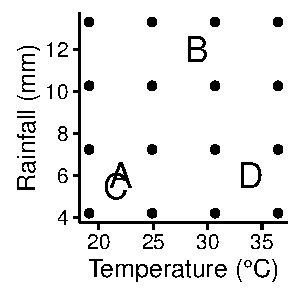
\includegraphics{figures_files/figure-latex/unnamed-chunk-3-1.pdf}
\caption{Attribute space example. This environmental attribute space has
dimensions relating to annual temperature (\(^{\circ}\)C) and rainfall
(mm). Letters denote the environmental conditions associated with the
geographic locations where four hypothetical populations are found.
Points represent demand points. In this space, populations close to each
other inhabit similar environmental conditions.}
\end{figure}

\begin{figure}
\centering
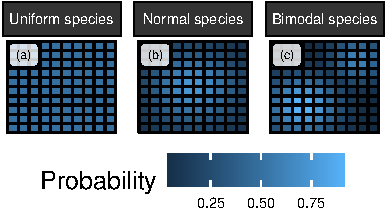
\includegraphics{figures_files/figure-latex/unnamed-chunk-4-1.pdf}
\caption{Distributions of three simulated species. Squares denote
planning units. Colors indicate probability of occupancy.}
\end{figure}

\begin{figure}
\centering
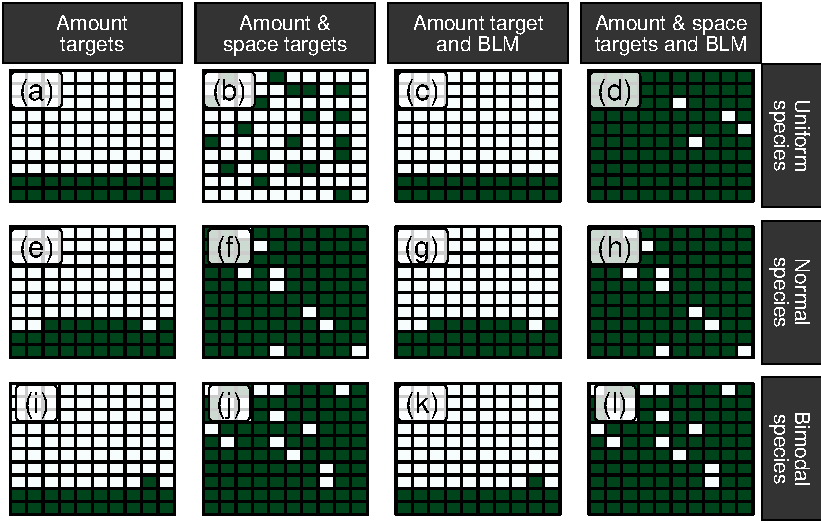
\includegraphics{figures_files/figure-latex/unnamed-chunk-5-1.pdf}
\caption{Prioritizations for the simulation study. Each panel shows a
prioritization generated for a single species using a set of parameters.
Squares denote planning units. Dark green planning units were selected
for protection. Each row of panels show prioritizations generated for a
different species. Each column of panels corresponds to a different set
of parameters used to generate the prioritization.}
\end{figure}

\begin{figure}
\centering
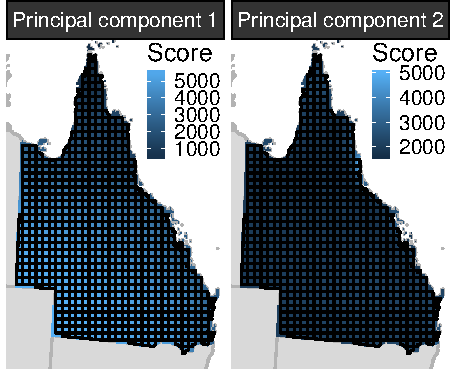
\includegraphics{figures_files/figure-latex/unnamed-chunk-6-1.pdf}
\caption{Two main gradients of climatic variation across Queensland,
Australia. Polygons denote planning units.}
\end{figure}

\begin{figure}
\centering
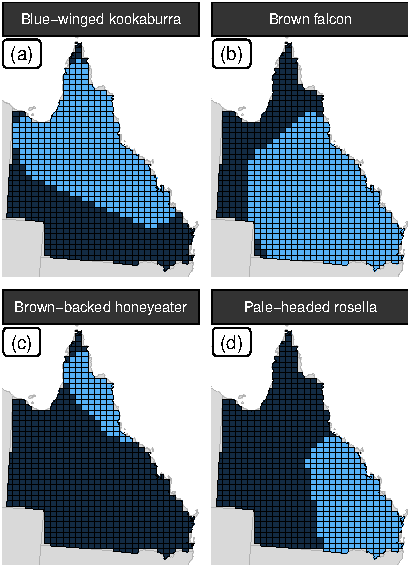
\includegraphics{figures_files/figure-latex/unnamed-chunk-7-1.pdf}
\caption{Distribution of the species used in the first case study.
Polygons denote planning units. Planning units occupied by a given
species are shown in light blue.}
\end{figure}

\begin{figure}
\centering
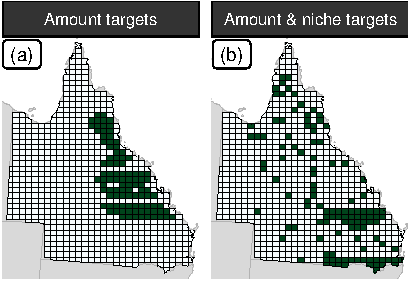
\includegraphics{figures_files/figure-latex/unnamed-chunk-8-1.pdf}
\caption{Prioritizations for the first case study. Polygons denote
planning units. Dark green planning units were selected for protection.
Panel (a) shows the solution generated when using 20 \% amount targets.
Panel (b) shows the solution when using 20 \% amount targets and -1e+06
\% niche targets.}
\end{figure}

\begin{figure}
\centering
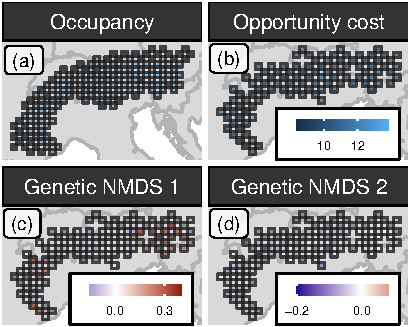
\includegraphics{figures_files/figure-latex/unnamed-chunk-9-1.pdf}
\caption{Data used for the second case study. Squares denote planning
units. Panel (a) shows all grid cells surveyed by the IntraBioDiv
project. Grid cells occupied by the betony-leaved rampion are shown in
bright blue. The subsequent panels contain only show occupied grid
cells. Panel (b) shows the acquisition cost of each planning unit
(estimated as the total human population density). Panels (c--d) show
the spatial distribution of the ordinations describing genetic
variation. These values describe the typical genetic characteristics of
individuals in each planning unit. Planning units with similar
values/colors contain individuals with similar loci polymorphisms.}
\end{figure}

\begin{figure}
\centering
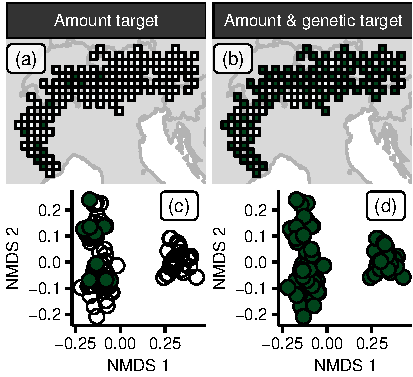
\includegraphics{figures_files/figure-latex/unnamed-chunk-10-1.pdf}
\caption{Prioritizations for the second case study. Panels (a--b) show
prioritizations generated using different parameters. Polygons denote
planning units. Dark green planning units were selected for protection.
Panel (a) shows the planning units selected when using 10 \% amount
targets. Panel (b) shows the planning units selected when using \%
amount targets and 85 \% genetic targets. Panels (c--d) show the
solutions in the genetic space. Each point corresponds to a planning
unit. The coordinates of the points represent the typical genetic
characteristics of individuals sampled in that planning unit (based on
an NMDS of the binary loci data). Planning units associated with points
that are closer together contain individuals with more similar genetic
characteristics than planning units that are further apart.}
\end{figure}



\end{document}
